\chapter{Human 3D pose from depth images}
%% WHAT IS IMPLEMETED
%% WHY DOES IT REPRESENT A PROGRESS IN RESEARCH

To train any network using supervised learning, large amounts of training data is needed. One of the goals for the \gls{mecs} project is to do \gls{har}, with the purpose of tracking a user from day to day, and look for patterns that could lead to worsening or more dangerous living conditions. The project also aims to be able to recognize the activity from any viewpoint, as the robot should be mobile to stay out of the way of the user as much as possible. A 2D approach to activity recognition will lack robustness or require training data from many different angles to complete this goal. A 3D approach will on the other hand provide robustness by not being dependent on the viewing angle.

This thesis focuses on describing a method for extracting human pose in 3D. By applying methods normally used on 3-channel (RGB) images to depth images, it is demonstrated that 

As in \cite{cao2017realtime}, two networks are used to create the \gls{paf}s and the confidence maps for the joints. However, instead of training on 3-channel RGB images, we will use a single channel depth image to discover the body landmarks/joints.
However, since depth images are single channel, and thus have less information than the RGB images, we propose using a shallower network. This also means we have to do the first step of feature extraction which was already done in a
However, since the depth images are less detailed than normal RGB images, some landmarks might be harder to detect: eyes, nose, or placing the joint on an outstretched limb.

This was considered when preparing the training data.

TODO> about not needing a full 3D body mesh, and privacy concerns

\section{Architecture}

TODO> about shallowness of network

The architecture of this project is \emph{recurrent} in that it repeats itself for a number of iterations. As with the architecture in \cite{cao2017realtime}, we have to have a first step which produces the first outputs we can use in later steps. However, this step is not illustrated in Fig.\ref{fig:arch_main}, since the first step will be identical to the next steps, except it will not have the additional inputs produced by the outputs of the previous step.

%% \begin{figure}[h]
%%   \centering
%%   \includegraphics[width=\textwidth]{img/architecture_main}
%%   \caption[Main architecture]{Main architecture. \gls{cnn}s are illustrated as hourglass networks, but this is not necessarily representative of the final architecture. A depth image is fed to a depth-feature extraction network (\ref{subsec:depth_feature}), which in consecutive steps are combined with output \gls{paf}s and joint confidence maps before this is fed to the 3D object detection networks (\ref{subsec:obj_detect}). These are run for a small number of iterations to get some estimate for the PAFs and confidence maps, before we move on to the assembly step. For each of the skeletons detected (with a ceiling for maximum detected skeletons) the skeletons with the strongest evidence are assembled. In the case that a body landmark is not found, we use preconceived coordinates from a standard defined skeleton. The coordinate frame of the skeleton in the articulation step till be the root joint (middle hip) with the z-axis pointing up, and the y-axis orthogonal to the line through the two side hip joints. The articulation network (\ref{subsec:articulation}) tries to scale and articulate the skeleton based on detected evidence. In the disassembly step, we place all the skeletons back into the camera coordinate frames, and update the \gls{paf}s and confidence maps with confidences and placements from the articulation network, and use them in the following steps. This is repeated a small number of times (3-4).}
%%   \label{fig:arch_main}
%% \end{figure}

\subsection{Depth feature extraction}\label{subsec:depth_feature}
For each pixel in the current layer of the \gls{cnn}, we collect information from a filter-sized portion of the previous layer. This means that deeper layers look at a larger and larger portion of the input layer. This is useful for detecting connections between large-scale structures. This also means that after a certain depth, there may not be any more useful information.

In our experiments, we will try different depths for feature extraction.

Some of these features might be desirable as inputs for later layers in object classification.

This network is built from the ground up. Therefore we want some layers to, for example, detect edges and one for detecting slanting gradients or connected surfaces. For limbs, we might want to find surfaces that are shaped like tubes or oblong spheroids.

\subsection{3D object detection}\label{subsec:obj_detect}
In this part of the network, we borrow some of the architecture described in \cite{cao2017realtime}. The purpose is to find joints and limbs and put them into \gls{paf}s or joint confidence maps. 

\subsection{Articulation network}\label{subsec:articulation}
The articulation network is stacked on top of the part-detection network and its main role is to refine the limb lengths and angles between each joint. Each of the detected persons are passed through the articulation network, which leads to a bit more complexity and runtime for the network based on the number of people. However, since the network has so comparatively few inputs, and is quite shallow, preformance is not expected to suffer notably.

The coordinates and confidences for each joint (if not detected, confidence is 0) and the mean PAF vector for each limb is the input to the network.

The network will try to find out what the positions of joints with low confidences, or no detections, should be. It is hypothesized that this network will learn things like symmetry (left and right limbs should have the same length), proportionality (limbs should be proportional to each other), possible articulations, and natural poses.

For joints that isn't detected or where the confidence is very low, the network will input some standard coordinates for that joint, scaled by the limbs we already have the strongest confidences for. The standard scaling/coordinates are hard-coded, based on the human anatomy surveys in \cite{bodySegmentParams}. The exception is eyes and ears, which is set to the best guess. In addition, the depth coordinate for each joint is set to 0. Numbering and a visualization of the skeleton can be seen in Figure \ref{fig:skeleton_markers}.

The architecture is visualized as a simple, fully connected neural network. Though, it might be enough to connect the neurons responsible for connected limbs. A neuron in the second layer connected to the foot, knee and one of the hip-joints does not need to be connected to the inputs from a hand or shoulder. Subsequent hidden layers can however, be fully connected.

If we had some input describing the direction of the camera, and the \gls{visual_hull} containing the undetected points, this network may perform better, because the position of the limb would be constrained to the \gls{visual_hull}. However, that would require a fundamental change to the network, which is not done in this work.

This network will also be trained separately, as all it needs is poses and random confidences as inputs.

\section{Training data preparation}

Skeleton models
\begin{figure}[h]

  \begin{floatrow}
    \ffigbox{
      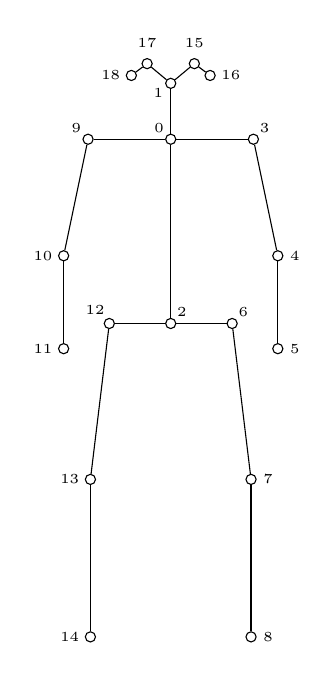
\begin{tikzpicture}[
          every node/.style={draw,circle,minimum size=.06cm, inner sep=1.3pt}
        ]
        \tiny
        %% \draw[help lines, step=5mm, gray!20] (-4,-4) grid (3,4);
        %% Standard coordinates => (orig.coords) - (0, .2)
        \node[label={[label distance=-.2mm]140:{0}}] (neck) at (0,2.54) {};
        \node[label={[label distance=-.2mm]200:{1}}] (nose) at (0,3.25) {};
        \node[label={[label distance=-.2mm]50:{2}}] (mhip) at (0, .2) {};

        \node[label={[label distance=-.2mm]50:{3}}] (lshoulder) at (1.05,2.54) {};
        \node[label={[label distance=-.1mm]0:{4}}] (lelbow) at (1.36,1.06) {};
        \node[label={[label distance=-.1mm]0:{5}}] (lwrist) at (1.36,-.12) {};
        \node[label={[label distance=-.2mm]50:{6}}] (lhip) at (.78,.2) {};
        \node[label={[label distance=-.1mm]0:{7}}] (lknee) at (1.02,-1.78) {};
        \node[label={[label distance=-.1mm]0:{8}}] (lankle) at (1.02,-3.78) {};

        \node[label={[label distance=-.2mm]140:{9}}] (rshoulder) at (-1.05,2.54) {};
        \node[label={[label distance=-.1mm]180:{10}}] (relbow) at (-1.36,1.06) {};
        \node[label={[label distance=-.1mm]180:{11}}] (rwrist) at (-1.36,-.12) {};
        \node[label={[label distance=-.2mm]140:{12}}] (rhip) at (-.78,.2) {};
        \node[label={[label distance=-.1mm]180:{13}}] (rknee) at (-1.02,-1.78) {};
        \node[label={[label distance=-.1mm]180:{14}}] (rankle) at (-1.02,-3.78) {};

        \node[label={[label distance=-.1mm]90:{15}}] (leye) at (.3,3.5) {};
        \node[label={[label distance=-.1mm]0:{16}}] (lear) at (.5,3.35) {};
        
        \node[label={[label distance=-.1mm]90:{17}}] (reye) at (-.3,3.5) {};
        \node[label={[label distance=-.1mm]180:{18}}] (rear) at (-.5,3.35) {};

        %% \draw[blue] (0,0) circle [radius=.06cm];

        \draw (nose) -- (neck);
        \draw (neck) -- (mhip);

        \draw (reye) -- (nose); \draw (leye) -- (nose);
        \draw (reye) -- (rear); \draw (leye) -- (lear);
        
        \draw (neck) -- (rshoulder); \draw (neck) -- (lshoulder);
        %% \draw (neck) -- (rhip); \draw (neck) -- (lhip);
        \draw (neck) -- (mhip);

        \draw (rshoulder) -- (relbow); \draw (lshoulder) -- (lelbow);
        \draw (rwrist) -- (relbow); \draw (lwrist) -- (lelbow);

        \draw (mhip) -- (rhip); \draw (mhip) -- (lhip);
        \draw (rhip) -- (rknee); \draw (lhip) -- (lknee);
        \draw (rknee) -- (rankle); \draw (lknee) -- (lankle);
      \end{tikzpicture}
    }
    {
      \caption[Numbering for keypoint markers]{Numbering for detected landmarks/keypoint markers.}
      \label{fig:skeleton_markers}
    }
    %% \end{figure}
    %% \begin{table}
    \capbtabbox{
      \footnotesize
      \begin{tabular}[H]{|r l r|}
        \hline
        \textbf{ID} & \textbf{Description} & \textbf{Std.Coord.} \\ \hline
        0  & Neck & (0.00, 2.34) \\
        1  & Nose & (0.00, 3.05) \\
        2  & Middle hip & (0.00, 0.00) \\
        3  & Left shoulder & (1.05, 2.34) \\
        4  & Left elbow & (1.36, 0.86) \\
        5  & Left wrist & (1.36, -0.32) \\
        6 & Left hip & (0.78, 0.00) \\
        7 & Left knee & (1.02, -1.98) \\
        8 & Left ankle & (1.02, -3.98) \\
        9  & Right shoulder & (-1.05, 2.34) \\
        10 & Right elbow & (-1.36, 0.86) \\
        11 & Right wrist & (-1.36, -0.32) \\
        12 & Right hip & (-0.78, 0.00) \\
        13 & Right knee & (-1.02, -1.98) \\
        14 & Right ankle & (-1.02, -3.98) \\
        15 & Left eye & (0.30, 3.30) \\
        16 & Left ear & (0.50, 3.15) \\
        17 & Right eye & (-0.30, 3.30) \\
        18 & Right ear & (-0.50, 3.15) \\
        \hline
      \end{tabular}
    }{
      \caption[Names/coordinates for detected landmarks]{Numberings, names/descriptions and standard coordinates for recognized landmarks}
      \label{tab:openpose_body_ids}
    }
  \end{floatrow}          
\end{figure}


\section{3D encoding}
The 3D scene is stored in a 2D depth map. That means that there is no need for a bounding box that creates constraints on how far away any detections can happen. The drawback being that any objects placed behind each other in the scene will suffer from being occluded.

Because of the 2D space, occurrences of distance information is limited to 1 per pixel in the 2D space. So, if two objects we want to represent are in line with each other (one occludes the other), there is no way to retain information about/distances to the two objects in the 2D space.
This leads to the question of how two inline (along the z-axis) joints can be represented for a 3D part affinity field. Even though for this use case, the only scenario is that two of the same limb is co-linear (i.e., two persons are standing right behind each other). This means that when parts are connected into skeletons, there will be a chance for a limb to be reused between two people.


TODO> explain targets for the CNN (limb- and joint-maps)
%% \section{2D detection transfer}

%% (First ideas.)

%% Torso placement and tree structure for placing.

%% Fit to human standard model (rules for symmetry and lengths)

%% Occlusion problem, and interpolated points, visual hull constraints

%% We train the network on both depth images and a kinematic model of each 3D ground truth location.

%% \section{Pose from CNN over depth maps}

%% We create a separate 'side-view' detection map for each 'frontal' detection map. This reduces the convolution operations, since we don't have to convolve over the whole 3D space.
